146. \begin{figure}[ht!]
\center{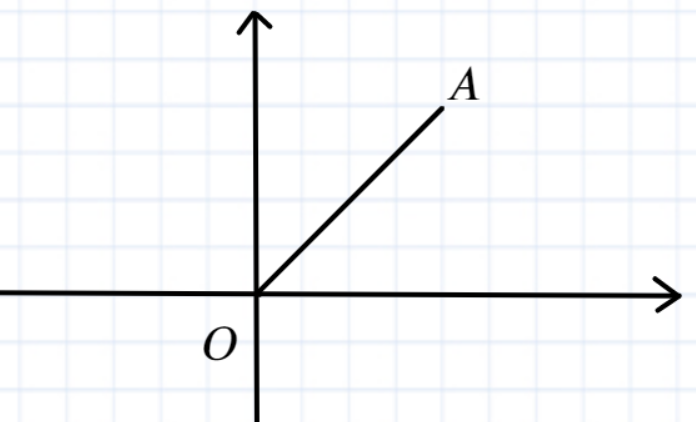
\includegraphics[scale=0.35]{g8-145.png}}
\end{figure}\\
Высота, опущенная из точки $O$ на $AB,$ равна 4. Тогда $S_{\Delta OAB}=\cfrac{1}{2}\cdot 4 \cdot AB=8,\ AB=4.$ Тогда абсцисса точки $B$ может быть равна либо $4+4=8,$ либо $4-4=0,$ то есть у точки $B$ могут быть координаты $(8;4)$ или $(0;4).$\\
